\chapter{Radioactive decay}
\textbf{$\alpha$ decay}: Occurs when the nucleus is unstable, due to being too big. The parent atom $\ch{^{A}_{Z}X}$ gets split into a daughter atom $\ch{^{A-4}_{Z-2}Y}$ and an alpha particle $\ch{^{4}_{2}a}$.\\
\textbf{$\beta^{-}$ decay}: Occurs when the nucleus is unstable, due to having an excess of neutrons. The parent atom $\ch{^{A}_{Z}X}$ gets split into a daughter atom $\ch{^{A}_{Z+1}Y}$, a beta particle $\ch{^{0}_{-1}e^{-}}$, and an anti-neutrino $\overline{v}_e$.\\
\textbf{$\beta^{+}$ decay}: Occurs when the nucleus is unstable, due to having an excess of protons. The parent atom $\ch{^{A}_{Z}X}$ gets split into a daughter atom $\ch{^{A}_{Z+1}Y}$, a positron $\ch{^{0}_{+1}e^{+}}$, and a neutrino $v$. After a number of interactions, the positron $\beta{+}$ unites with an electron and converts its entire mass to energy. This annihilation produces 511 keV.\\
\textbf{Electron capture}: The nucleus absorbs an electron from the electron cloud (usually from shell K -innermost). The parent atom $\ch{^{A}_{Z}X}$ absorbs an electron $\ch{^{0}_{-1}e^{-}}$, and gets split into a daughter atom $\ch{^{A}_{Z-1}Y}$, and a neutrino $v$.\\
\textbf{Gamma decay ($\gamma$)} Occurs when the atom is excited. The parent atom $\ch{^{A}_{Z}X*}$ gets excited and produces a daughter particle $\ch{^{A}_{Z}X}$ and a gamma ray $\gamma^{1}$. Internal conversion may occur (direct transsfer of the energy of the nucleus to an electron).
%--------------------------------------------------------------------------------------------------------------------------------------------------------------------------------------------------------------------------------------------------------------------------------------------------------------------------%
\chapter{Formulas}
\section{Activity determination}
\[A(t) = A(0) \cdot (\frac{1}{2})^{\frac{t}{T_{1/2}}}\]
\textbf{Precise determination with a formula for the half-life using half-life}. All time units must be in the same unit.\\
\[\frac{dN(t)}{dt}=-\lambda\cdot N(t);\ A(t) = A(0)\cdot e^{-\lambda t}\]
\textbf{Precise determination with a formula for the half-life using decay constant ($\lambda$)}. All time units must be in the same unit.\\

\section{Shielding}
\[g \approx 2\cdot10^{-4}\cdot Z\cdot E_{\beta,max}\]
\textbf{Approximation of the energy converted to Bremsstrahlung}. Where $Z$ is the atomic number of the shielding material\\
\[R_{\beta,\ in\ material} = \frac{R_{\beta,\ in\ water} = 0.5 E_{\beta,max}}{\rho_{material}}\]
\textbf{Range of $\beta$ particle in a specific material}. For water and tissue, $\rho$ can be estimated to be 1 g/cm³. $E_{\beta,max}$ is expressed in MeV.\\
\[I(d) = I(0)\cdot B\cdot(\frac{1}{2})^{\frac{d}{d_{1/2}}}\]
\textbf{Shielding of $\gamma$ radiation using half distance}. Buildup factor (P60) may be ignored. All distance units must be in the same unit.\\
\[I(d) = I(0)\cdot e^{-\mu_{linear} d}; \mu_{mass} = \mu_{linear}\cdot\rho_{material}^{-1}\]
\textbf{Shielding of $\gamma$ radiation using linear attenuation coefficient}. Above 500keV, $\mu_{mass\ water}\approx\mu_{mass\ concrete}$.\\

\section{Dose determination}
\[H_T = W_R \cdot D\]
\textbf{Equivalent dose}. $W_R$ is the radiation weighting factor: 1x for $\beta$ and $\gamma$, 20x for $\alpha$, and 2-20x for $N_0$. D is the absorbed dose over tissue of organ (Gy).\\
\[E = \sum (W_T \cdot H_T)\]
\textbf{Effective dose}. $W_T$ is the tissue weighting factor (P64). \\
\[E(50) = e(50)\cdot A\]
\textbf{Committed effective dose (Sv)}. e(50) is the committed effective dose coefficient (Sv$\cdot$Bq$^{-1}$).\\
\[\cdot H*(10) = h(10)\cdot\frac{A}{r²}\]
\textbf{Inverse square law}. The activity must be in MBq, the distance in m, and the result in $\mu$Sv/h\\
\[X\]
\textbf{}\\

\section{Measurement}
\[rel. error = \frac{\sqrt{N}}{N} = \frac{1}{\sqrt{N}}\]
\textbf{Relative error}. $N$ is the number of counted pulses, $\sqrt{N} is the counting error$\\
\[\epsilon = \frac{R}{A}\]
\textbf{Efficiency}, where R is the counting rate in units of per second, and A is the activity in Bq.\\
%--------------------------------------------------------------------------------------------------------------------------------------------------------------------------------------------------------------------------------------------------------------------------------------------------------------------------%
\chapter{Useful information}
\begin{figure}
    \centering
    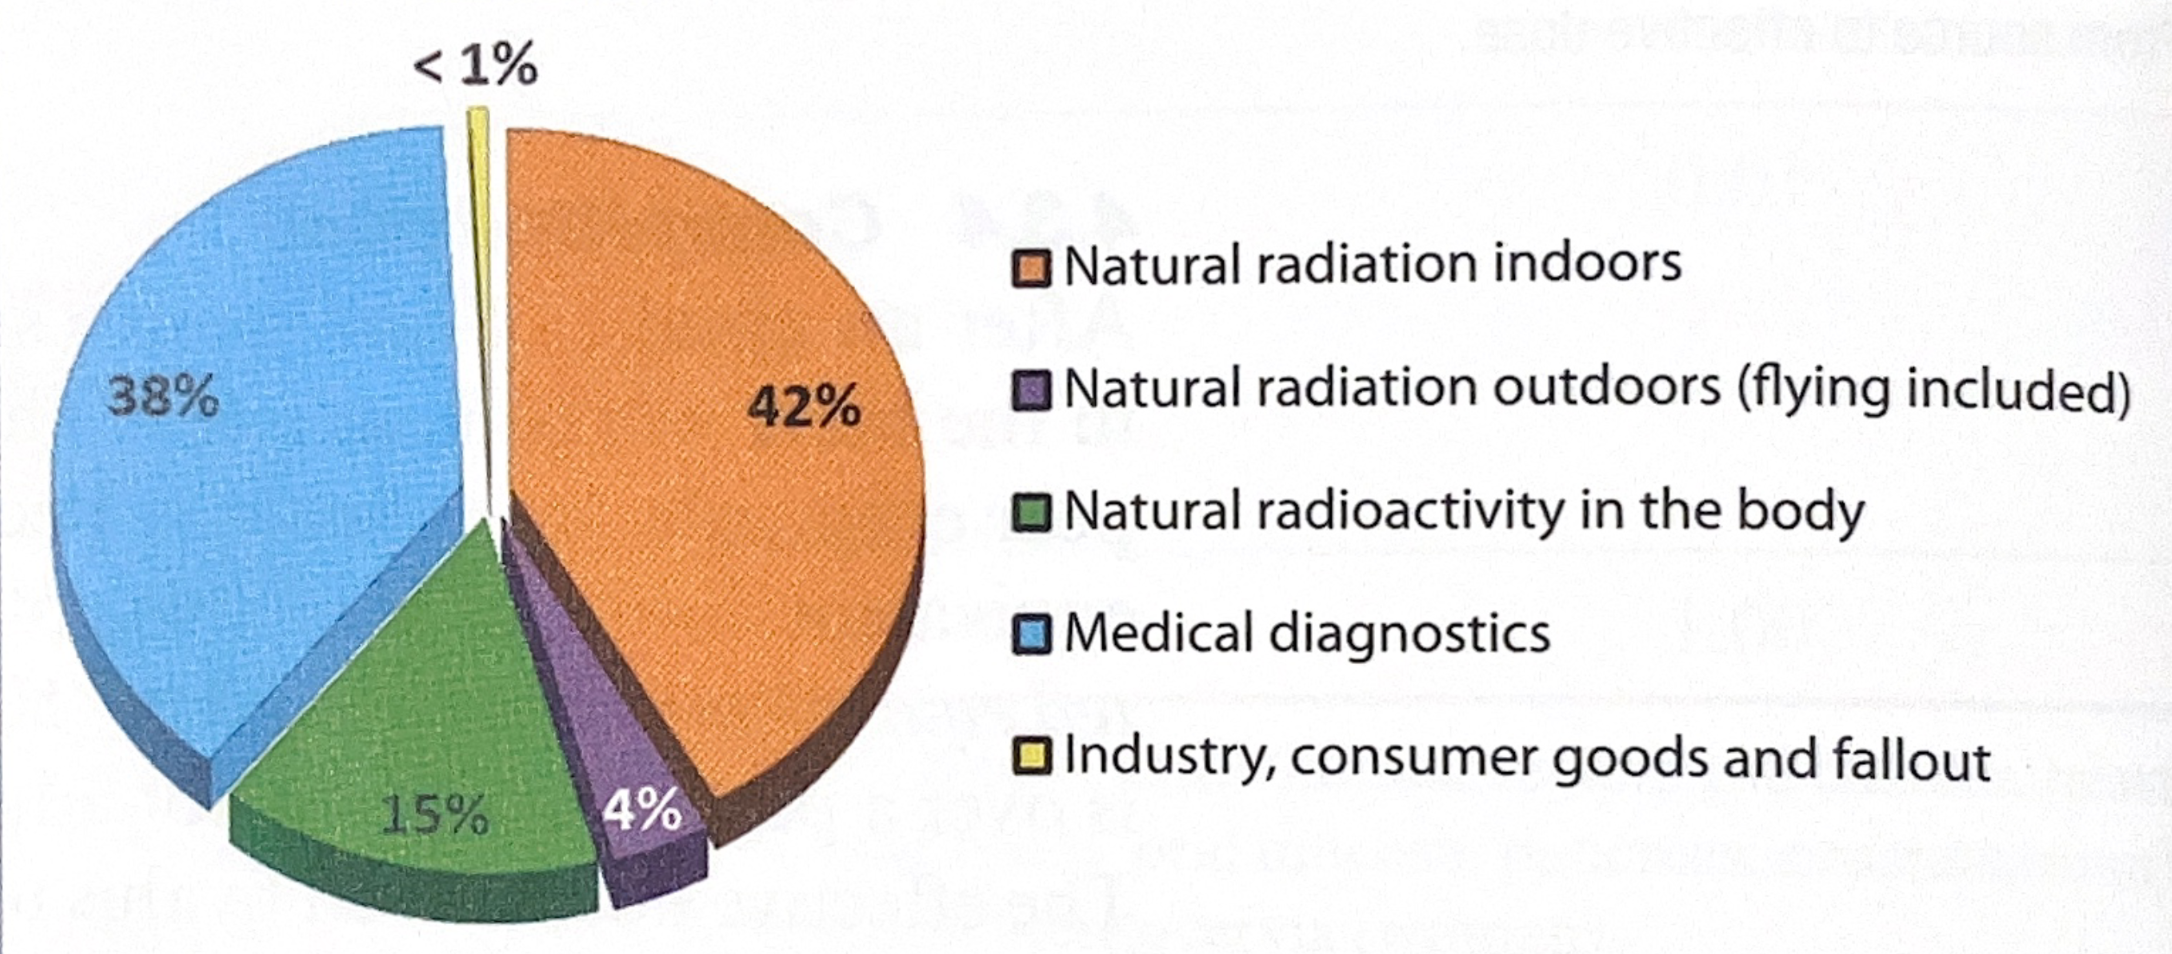
\includegraphics[width=0.5\linewidth]{Normal_dose.png}
    \caption{Contributions to the dose for a member of the public in the Netherlands}
    \label{fig:placeholder}
\end{figure}
%$$$$$$$$$$$$$$$$$$$$$$$$$$$$$$$$$$$$ TODO: Add figures: 4.2
\begin{table}[ht]
\caption{Detectors and their usual applications}
\label{detect}
\begin{tabular}{lll}
\hline
 & $\beta$ emitters & Photon radiation \\ \hline
\textbf{Ionisation detectors} &  &  \\
GM Tube (thin window) & Contamination & Contamination \\
GM Tube (thick window) & - & Dose rate \\
Proportional counter (thin window, xenon filled) & Large area contamination & Large area contamination \\for low-energy photons \\
Germanium semiconductor & - & Accurate spectrum \\ \hline
\textbf{Scintillation detectors} &  &  \\
Nal(Tl) & - & \begin{tabular}[c]{@{}l@{}}Contamination\\ Simple spectrum\\ Dose rate\end{tabular} \\
Andthracene or ZnS & Contamination & Contamination \\
TLD & Personal dosimeter & Personal dosimeter \\
 &  & 
\end{tabular}
\end{table}
%----------------------------------%
\begin{table}[ht]
\caption{Dose limits}
\label{doses}
\begin{tabular}{llll}
\rowcolor[HTML]{343434} 
\multicolumn{1}{l|}{\cellcolor[HTML]{343434}{\color[HTML]{FFFFFF} \textbf{Group}}} & \multicolumn{1}{l|}{\cellcolor[HTML]{343434}{\color[HTML]{FFFFFF} \textbf{\begin{tabular}[c]{@{}l@{}}Effective dose [mSv/y]\end{tabular}}}} & \multicolumn{2}{l}{\cellcolor[HTML]{343434}{\color[HTML]{FFFFFF} \textbf{\begin{tabular}[c]{@{}l@{}}Equivalent dose [mSv/y]\end{tabular}}}} \\
\rowcolor[HTML]{C0C0C0} & \multicolumn{1}{l|}{\cellcolor[HTML]{C0C0C0}{\color[HTML]{333333} Total body}} & \multicolumn{1}{l|}{\cellcolor[HTML]{C0C0C0}{\color[HTML]{333333} Eye lens}} & {\color[HTML]{333333} Skin \& extremities} \\ \hline
\textbf{Category A} & 20 & 20 & 500 \\
\textbf{\begin{tabular}[c]{@{}l@{}}Category B\\ Exposed pupils and students\\ Those between 16 and 18\end{tabular}} & 6 & 15 & 150 \\
\textbf{\begin{tabular}[c]{@{}l@{}}Category C\\ ``Non-exposed employees''\end{tabular}} & 1 & 15 & 50 \\
\textbf{Pregnant employees} & \multicolumn{3}{l}{Maximum 1 mSv equiv to abdomen from announcement to birth.} \\
\textbf{\begin{tabular}[c]{@{}l@{}}Members of the public\\ Excluding patients\end{tabular}} & 1 & 15 & 50
\end{tabular}
\end{table}































\[X\]
\textbf{}\\